% 2011 山东卷(文) 第22题 图: 椭圆与直线(单圆锥曲线+少量直线)
\usetikzlibrary{arrows.meta,calc}
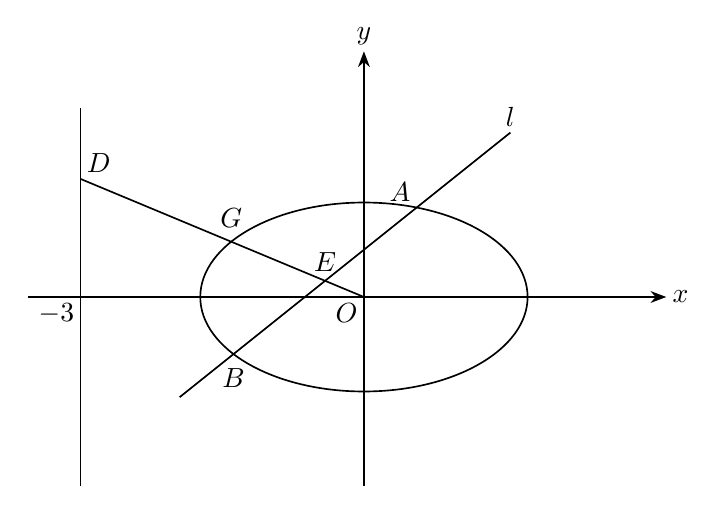
\begin{tikzpicture}[x=1cm,y=1cm,line width=.6pt,font=\normalsize,>=Stealth]
%==DATA-START== do not reorder
\def\scale{1.2}
\def\ellRx{2.0784609690826525}
\def\ellRy{1.2}
\coordinate (O) at (0.0,0.0);
\coordinate (A) at (0.6699428792946497,1.1359543034357198);
\coordinate (B) at (-1.6562442491576634,-0.7249953993261308);
\coordinate (E) at (-0.4931506849315069,0.20547945205479454);
\coordinate (G) at (-1.68539251962428,0.7022468831767833);
\coordinate (D) at (-3.6,1.5);
\coordinate (Lone) at (-2.34,-1.272);
\coordinate (Ltwo) at (1.86,2.088);
\coordinate (Xone) at (-4.26,0.0);
\coordinate (Xtwo) at (3.84,0.0);
\coordinate (Yone) at (0.0,-2.4);
\coordinate (Ytwo) at (0.0,3.12);
\coordinate (Vone) at (-3.6,-2.4);
\coordinate (Vtwo) at (-3.6,2.4);
%==DATA-END==
\draw[->] (Xone)--(Xtwo) node[right=2pt,inner sep=0pt] {$x$};
\draw[->] (Yone)--(Ytwo) node[above=2pt,inner sep=0pt] {$y$};
\draw (Vone)--(Vtwo);
\draw (O) ellipse ({\ellRx} and {\ellRy});
\draw (Lone)--(Ltwo);
\draw (O)--(D);
\node[below left,inner sep=0pt,xshift=-2pt,yshift=-2pt] at (O) {$O$};
\node[above left,inner sep=0pt,xshift=-2pt,yshift=2pt] at (A) {$A$};
\node[anchor=north,inner sep=0pt,yshift=-5pt] at (B) {$B$};
\node[above,inner sep=0pt,yshift=3pt] at (E) {$E$};
\node[anchor=south,inner sep=0pt,yshift=5pt] at (G) {$G$};
\node[above right,inner sep=0pt,xshift=2pt,yshift=2pt] at (D) {$D$};
\node[below left,inner sep=0pt,xshift=-2pt,yshift=-2pt] at (Vone |- Xone) {$-3$};
\node[above,inner sep=0pt,yshift=2pt] at (Ltwo) {$l$};
\end{tikzpicture}
